\section{Numerical Setup and Results}

In this Section we first introduce the experimental setup used to run the
closure tests, and then discuss the actual results. Following the study performed in 
Ref.~\cite{nnpdf30}, we first analyse the relative 
size of the different components of PDFs uncertainty, comparing the changes between the old
and the new methodologies, used to produce the NNPDF3.1 \cite{Ball_2017} and NNPDF4.0 \cite{NNPDF40} 
sets of PDFs respectively. We then move to the data space estimators $\biasvarratio$ and $\xisigdat{1}$,
which have been computed only for NNPDF4.0
\footnote{as pointed out before, the computation of the expectation value over training data,
defined in Eq.~\ref{eq:average_over_training_data}, is made possible by the efficiency of the new code \cite{nnpdf40code}.}.
The results here act both as a proof of principle of new estimators presented in this paper but also
as part of a suite of methodological validation tools, see also the "future
tests" \cite{Cruz_Martinez_2021}, used to understand the PDF uncertainties of
the recent NNPDF4.0 set of PDFs. For the purpose of understanding how the
results here were produced, we will briefly describe the key features of the
NNPDF4.0 methodology, but refer the reader to NNPDF4.0 for a full discussion on
how these methodological choices were made, and the impact on performing PDF
fits to experimental data.

\subsection{Closure test setup}

Using neural networks to fit PDFs has been discussed many times in previous
NNPDF publications, see for example \cite{nnpdf30, Ball_2017}. A new feature of
NNPDF4.0 is that, for the default fit performed in the evolution basis, a
single neural network parameterises all 8 PDF flavours $\{ g, \Sigma, V, V_3,
V_8, T_3, T_8, T_{15} \}$ at the initial scale. The PDF for a single flavour $j$,
at the initial scale $Q_0 = 1.65~{\rm GeV}$ is given by
\begin{equation}
    f_j(x, Q_0) = NN(x, \ln x | \modelvec)_j * x^{1-\alpha_j} * (1-x)^{\beta_j},
\end{equation}
where $\alpha$ and $\beta$ are the preprocessing exponents, which control the
PDF behaviour at $x \to 0$ and $x \to 1$ respectively and $NN(x, \ln x |
\modelvec)_j$ is the $j^{\rm th}$ output of the neural network, which takes $x$
and $\ln x$ as input. As discussed in Sec.~\ref{sec:fit-reps}, an ensemble of
models is fitted, each one is a MAP estimator of the corresponding pseudo-data
it is fitted on. 
An optimization algorithm is used to try and find the parameters which maximise the likelihood.
In principle, the preprocessing exponents can also be varied during the fit
analogously to the neural network parameters, such as in \cite{Carrazza_2019},
or they can be randomly selected from a predetermined range as is done in
previous NNPDF releases, for example \cite{Ball_2017}. There are clearly many
choices with respect to hyperparameters, the discussion of how these choices
have been made is beyond the scope of this paper and left to the full NNPDF4.0
release \cite{NNPDF40}. A summary of the hyperparameters used to produce results
presented in this paper are provided in Tab.~\ref{tab:Hyperparams}.


As input to the closure test, a single replica was drawn randomly from a
previous NNPDF fit to experimental data. We refer to this as the underlying law
and the corresponding predictions the true observable values. An example of the
gluon input is provided in Fig.~\ref{fig:InputGluonPDF}. In principle any
function could be used as underlying law, however it makes sense to use a
realistic input.

\begin{figure}
    \centering
    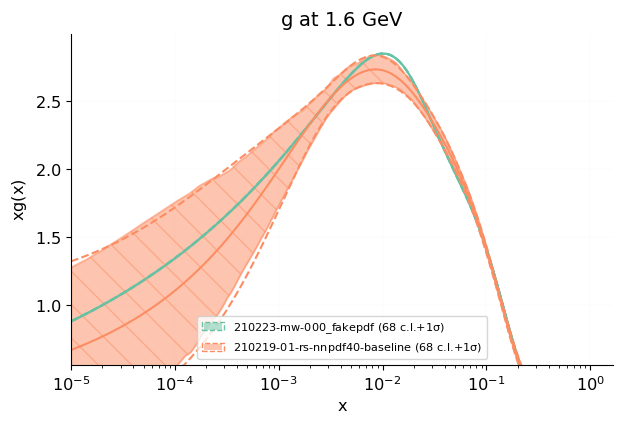
\includegraphics[width=0.8 \textwidth]{plot_pdfs_g.png}
    \caption{The green line is the input underlying law for the gluon PDF,
    which is sampled from the ensemble from a fit to data. The 68\% confidence
    interval is plotted for those replicas as the orange band.}
    \label{fig:InputGluonPDF}
\end{figure}

The observables used in the fits are a subset of the full NNPDF4.0 dataset. For
convenience, we chose to fit the PDFs on a variant of the NNPDF3.1 dataset used
in Ref.~\cite{Ball_2018}, which is described in detail in a study of the
determination of the strange PDF~\cite{Faura_2020}. 
The datasets used in the
calculation of statistical estimators are the new datasets which will be
included in NNPDF4.0, which will be discussed in detail with the main release.
For a full summary of observables used in the test data and a visual
representation of the kinematic region of both the training and testing data,
see App.~\ref{sec:appendix-datasets}.

The choice of data for both fitting and testing is considered unimportant, one
could consider splitting the data into training and test in a way which
considered kinematic coverage rather than this naive chronological splitting.
Alternatively, since the data is generated from the theory predictions produced
by the input underlying law, one could even produce completely artificial data
using a different set of FK tables. From a practical standpoint, using the
NNPDF3.1 dataset and validating on the newly included datasets in 4.0 allowed us
to validate the PDF uncertainties on data outside of the kinematic coverage of
data included in the fit. Furthermore, the data estimators only give us local
information on the PDF uncertainties and it seems logical to split the data in
this way since the results seem more applicable to the reality of how the PDFs
end up being used.

In order to compute the expectation value over training data defined in Eq.~\ref{eq:average_over_training_data},
we generate 30 different sets of experimental central values (or L1 data),
as discussed in Sec.~\ref{sec:closure-test-intro}, for the fitted 3.1-like
dataset. Each set of experimental central values was then fitted following
NNPDF4.0 methodology \cite{NNPDF40}, producing 40 pseudo-data replicas.


\subsection{Different components of the PDF uncertainty}

As already discussed in Ref.~\cite{nnpdf30}, fitting to L0, L1 and L2
pseudo-data allows us to validate different aspects of the fitting procedure. In
an L0 fit, we fit multiple time the exact same set of data, which corresponds to
the theory prediction from the chosen model. The fitted pseudo-data is the
result obtained by applying the forward map to the model. It is clear that in
this case the quality of the fit can be improved at will, provided that the
parametrization is flexible enough and the minimization algorithm is efficient.
There are indeed multiple solutions that reproduce exactly the data set, while
interpolating between the data points. In an L1 the data have been fluctuated
around the theoretical prediction -- mimicking thereby the central values of
experimental measurements. The true model no longer reproduces the data; instead
it will yield a $\chi^2$ of order one. The pseudo-data are held fixed,
fluctuations from one replica to the next are due to the existence of multiple
solutions that hold a similar value for the residual $\chi^2$ at the end of the
minimization process. Finally, in the L2 fits, the fluctuations of the data are
reproduced by the replicas, and propagated to the model function when fitting
the data for each replica. Since the NNPDF fitting methodology has changed in
the latest release, it is important to compare the uncertainties at L0, L1 and
L2 that are obtained with the new fitting routine with the corresponding
ones obtained with the old fitting code. 

An example of these relative errors on fitted PDFs is shown in Fig.~\ref{fig:CT_uncertainty_g} 
where results from L0, L1 and L2 closure tests are displayed on the same plot in the case of the gluon distribution.
Each fit is normalized to the corresponding central value. 
We note how the L0 and L1 uncertainties tend to increase in the $x$ regions where less experimental data are available,
namely at small and large-$x$, where the model is left unconstrained and has more freedom to fluctuate,
while they are considerably reduced in the data region 
where the contribution of the L2 error, induced by the actual experimental data, becomes more important.
The fact that the data uncertainty is not always the dominant component of the PDF uncertainty
was already stressed in Ref.~\cite{nnpdf30}. Improved methodologies should therefore aim to reduce the L0 and L1
error. 

In this respect, it is interesting to compare these results with what we find with the old fitting code. The corresponding
plots are shown in Fig.~\ref{fig:CT_uncertainty_g_nnpdf3.1}: unlike the NNPDF4.0 case, here the PDF uncertainty 
is always dominated by the L0 uncertainty, even in those kinematic regions where experimental data are present.
We can conclude that moving to the new methodology we observe a marked reduction of the L0 uncertainty.
This, most likely, is due to the optimized architecture and the different minimizer used in NNPDF4.0, 
which has been proved to be much more efficient than the genetic algorithm, adopted in the previous NNPDF determinations.
This can be appreciated by looking at Fig.~\ref{fig:chi2_vs_epoch},
where we plot the $\chi^2$ distribution across replicas as a function of the training epoch for the L0 closure tests
in the new and old methodology. As mentioned before, in a L0 closure test the quality of the fit can in principle be improved at will,
assuming the use of an efficient optimizer.
For the final $\chi^2$ of the central value of each fit, plotted as a black dashed line, 
we find $0.002$ and $0.012$ in the new and old fitting code respectively,
showing the better efficiency of the new methodology. 

It should be noted how Figs.~\ref{fig:CT_uncertainty_g},~\ref{fig:CT_uncertainty_g_nnpdf3.1} only provide a qualitative assessment of the relative size of the different
components of PDFs uncertainty. Despite being useful to assess how the methodology has improved with respect
to the previous one, they do not provide any quantitative estimation of the faithfulness of PDF uncertainty.
This can only be done in data space, using the new estimators introduced in the previous sections.

\begin{figure}[h]
    \centering
    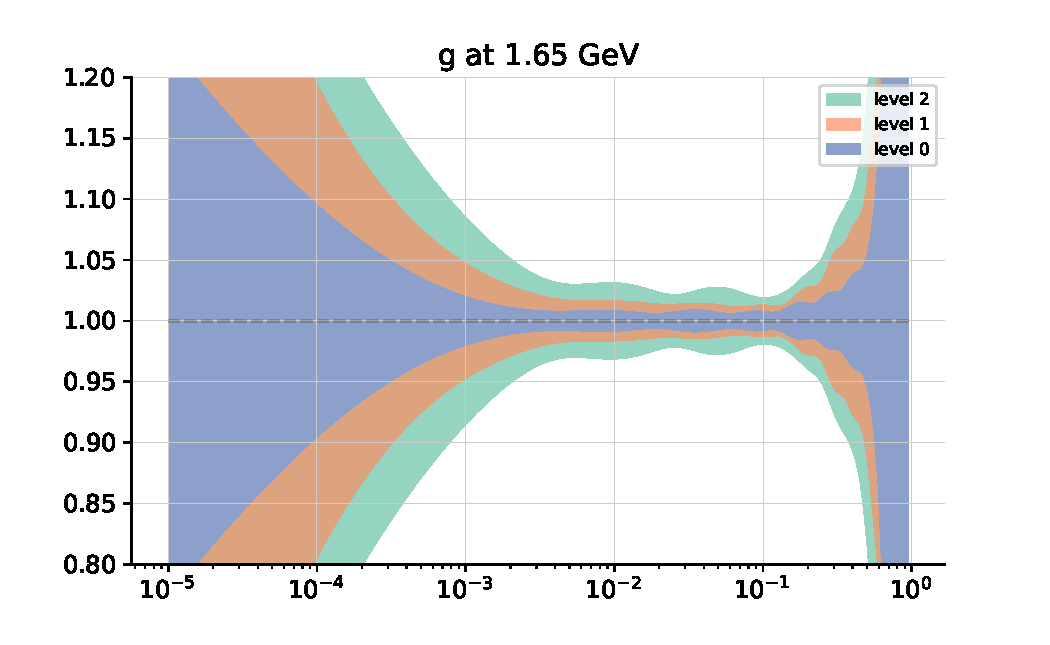
\includegraphics[scale=0.43]{CT_log_g.pdf}
    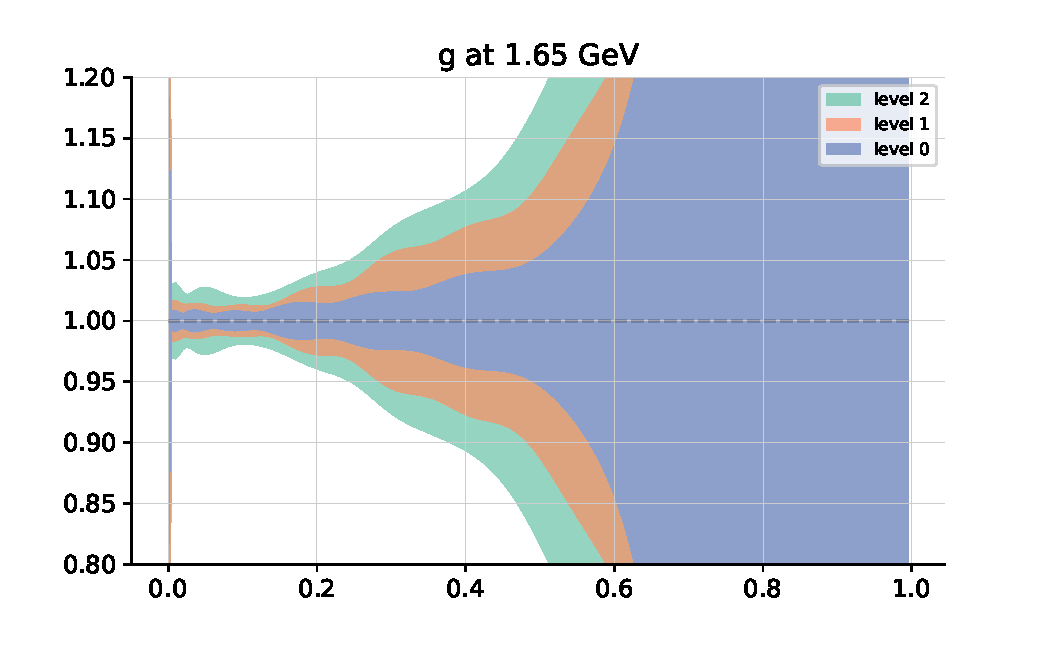
\includegraphics[scale=0.43]{CT_linear_g.pdf}
    \caption{Relative PDF error for the gluon distribution in the new methodology,
    plotted in logarithmic (left) and linear scale (right).}
    \label{fig:CT_uncertainty_g}    
\end{figure}

\begin{figure}[h]
    \centering
    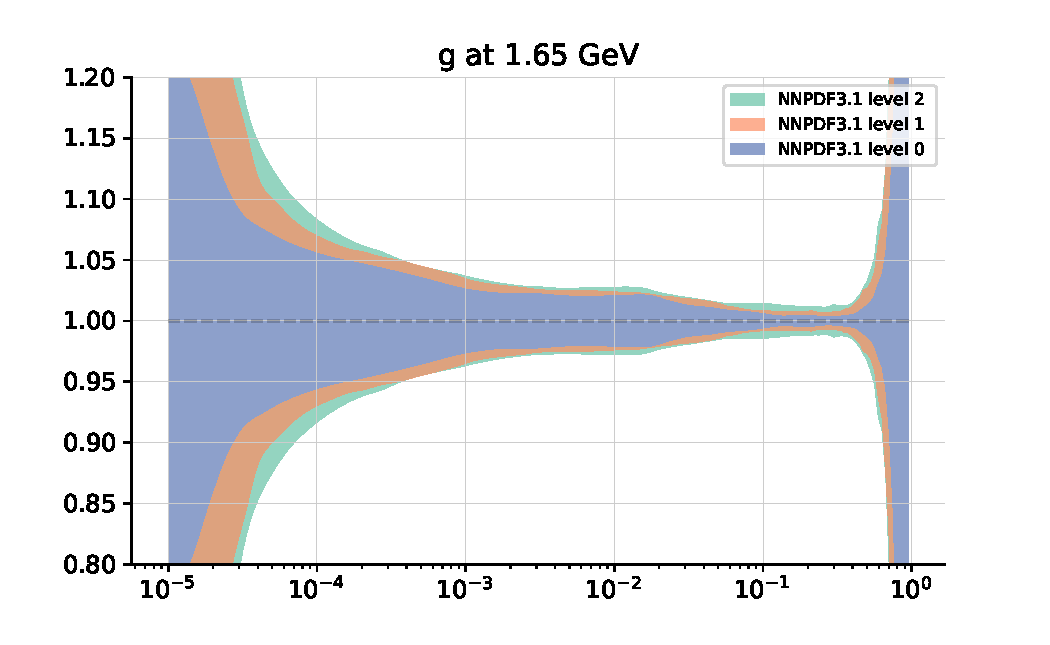
\includegraphics[scale=0.43]{CT_log_g_nnpdf31.pdf}
    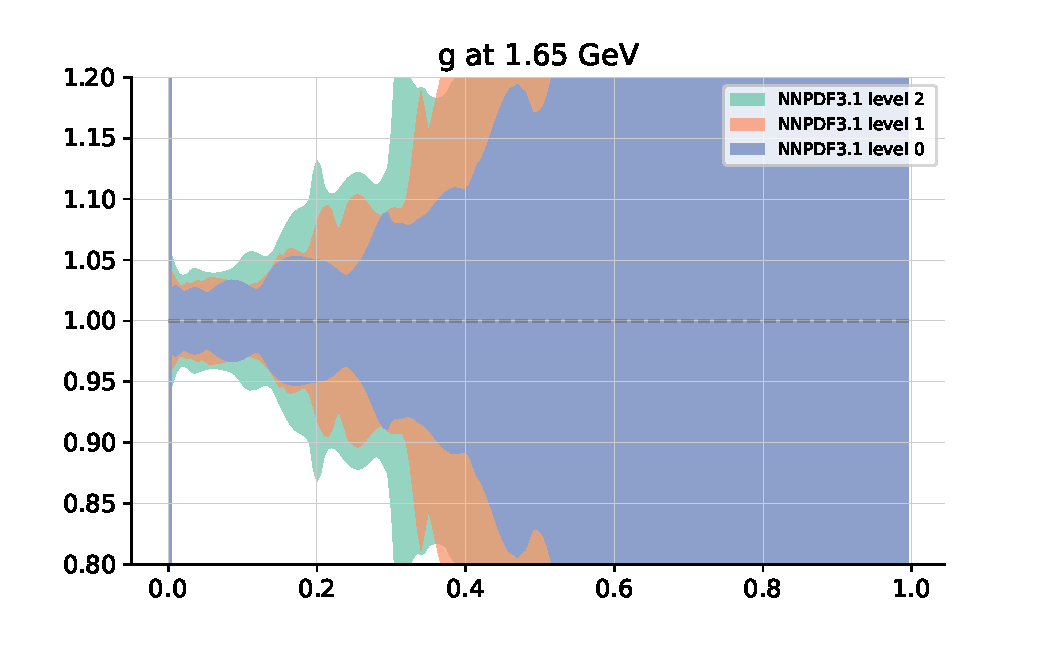
\includegraphics[scale=0.43]{CT_linear_g_nnpdf31.pdf}
    \caption{Same as Fig.~\ref{fig:CT_uncertainty_g} for the old methodology.}
    \label{fig:CT_uncertainty_g_nnpdf3.1}    
\end{figure}

\begin{figure}[h]
    \centering
    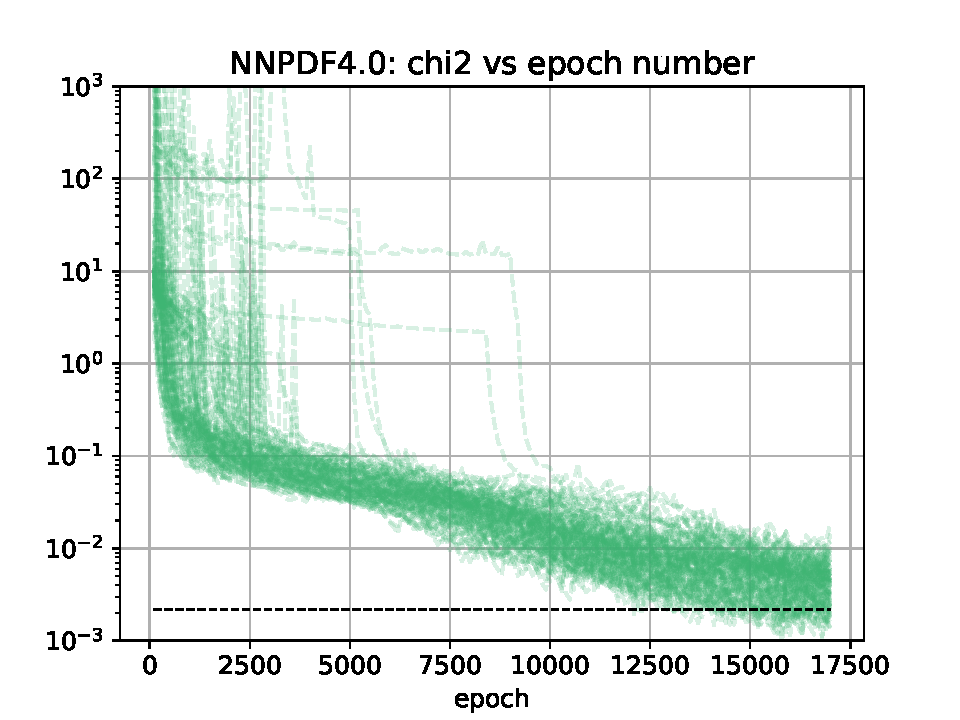
\includegraphics[scale=0.43]{chi2_n3fit_L0.pdf}
    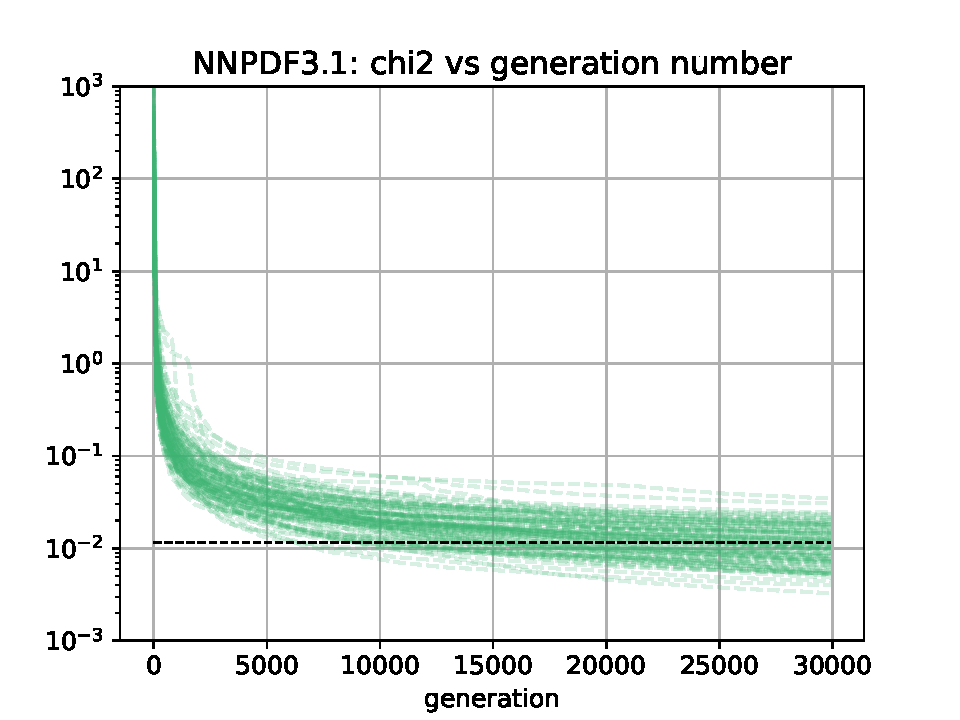
\includegraphics[scale=0.43]{chi2_nnfit_L0.pdf}
    \caption{$\chi^2$ distribution across replicas as a function of the training epoch for the new (left)
    and old (right) methodology. The black dotted line in each plot represents the final 
    $\chi^2$ of the central value of the corresponding fit, equal to $0.002$ and $0.012$ respectively.}
    \label{fig:chi2_vs_epoch}    
\end{figure}



\subsection{Data space estimators}

Results for $\biasvarratio$ and the corresponding uncertainty calculated on the test data are shown in
 the first column of Tab.~\ref{tab:biasvarratio}. These have been computed by performing a bootstrap sample
\cite{efron1994introduction}, where we randomly sample from both fits and replicas and re-calculate
$\biasvarratio$. The value and error presented in the table is then the mean
and standard deviation across bootstrap samples. We checked that the distribution
of the estimator across bootstrap samples is indeed Gaussian. We also checked
that increasing the number of fits and replicas reduced the bootstrap error but
the central values were the same within the estimated bootstrap uncertainties. 
We see that overall $\biasvarratio$  is consistent with 1, which
gives a good indication that, at least for the unseen data used in this study, the uncertainties are
faithful

\begin{table}[h]
    \begin{center}
        \setlength{\tabcolsep}{12pt} 
        \begin{tabular}{rrr}
            \toprule
             $\biasvarratio$ & $\xi_{1\sigma}$ & $\erf(\biasvarratio/\sqrt{2})$ \\
            \midrule
             $1.03\pm0.05$ & $0.69\pm0.02$   & $0.67\pm0.03$                  \\
            \bottomrule
            \end{tabular}
    \end{center}
    \caption{
        In the first column we show the bias-variance ratio, $\biasvarratio$, for unseen data, summarised in
        Tab.~\ref{tab:summarise_new_data}. The uncertainty is estimated by
        performing a bootstrap sample across fits and replicas and calculating
        the standard deviation. We see that overall $\biasvarratio$ is consistent
        with 1, within uncertainities. 
        In the second and third columns we compare the measured value of $\xi_1\sigma$ and the estimated
        value from $\biasvarratio$. The two values are consistent, which
        suggests the approximation that the ratio of uncertainties is
        approximately the same across all data is not completely invalidated.
    }
    \label{tab:biasvarratio}
\end{table}

In Fig.~\ref{eq:bias_varinace_distributions} we compare qualitatively the distribution 
of bias across fits, to the
distribution of the difference between replica predictions and expectation
values of predictions (in units of the covariance) across different fits
and replicas. The square root ratio of the mean of these two distributions
is precisely $\biasvarratio$.

\begin{figure}[h]
    \centering
    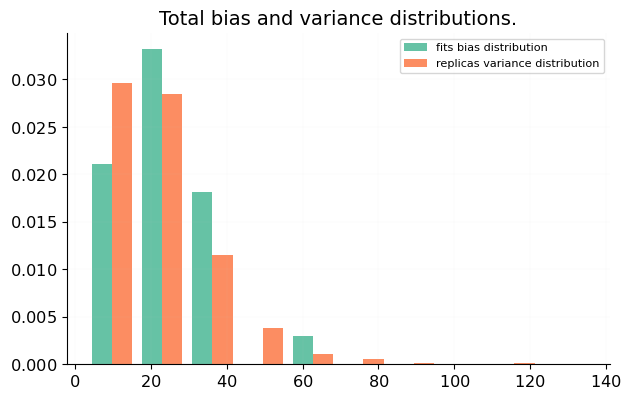
\includegraphics[width=0.6 \textwidth]{plot_bias_variance_distributions_total.png}
    \caption{The green histogram is the distribution of the total bias across fits,
    the orange histogram is the distribution of the difference between the
    replica and central predictions squared, in units of the covariance
    across all fits and replicas. This gives a qualitative picture of the full
    distribution, in Tab.~\ref{tab:biasvarratio} we compare the square root of the
    mean of each distribution, getting the quoted value for $\biasvarratio$.}
    \label{eq:bias_varinace_distributions}
\end{figure}

As discussed in Sec.~\ref{sec:QuantileStatistics}, one can define an analogous
estimator in data space, based upon $\xi_{n\sigma}$, which was defined on a grid
of points in $x$ and $Q^2$ in PDF space in \cite{nnpdf30}. There is not
a one-to-one correspondence
between this and $\biasvarratio$, but a loose approximation using
Eq.~\ref{eq:expectedxi}. In the second and third columns of Tab.~\ref{tab:biasvarratio} we compare the estimated
$\xi_{1\sigma}$ from
subsituting $\biasvarratio$ into Eq.~\ref{eq:expectedxi} and to the
measured value.
Despite the assumptions entering each of the two estimators differing, we see
good agreement between the $\xi_{1\sigma}$ estimated from $\biasvarratio$
and that measured directly. We find this result reassuring, since it indicates
not only that the total uncertainty averaged across all data is faithful, but
also that the uncertainty on each data point seems faithful. If the results
differed it would indicate some kind of imbalance, where some components
of the uncertainty are correctly represented by the replicas but other directions
are not. Finally we note how not only are the measured value and estimated value from $\biasvarratio$
self consistent, but they are also consistent with $0.68$, which
further supports the argument that the model uncertainties are
faithful.

\iffalse
\begin{figure}[ht]
    \centering
    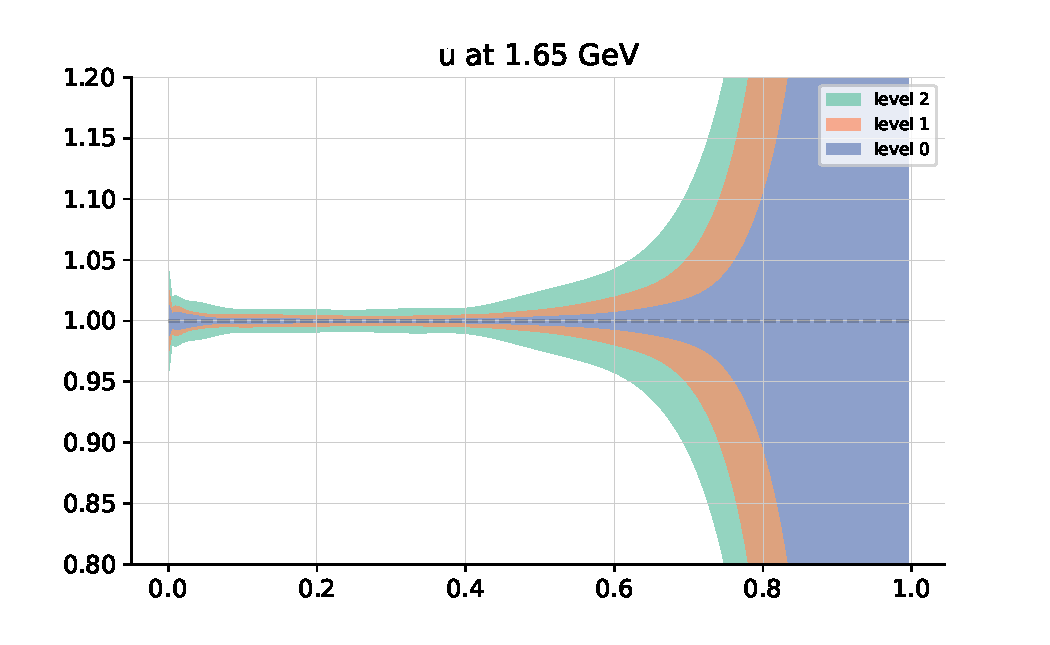
\includegraphics[scale=0.43]{CT_linear_u.pdf}
    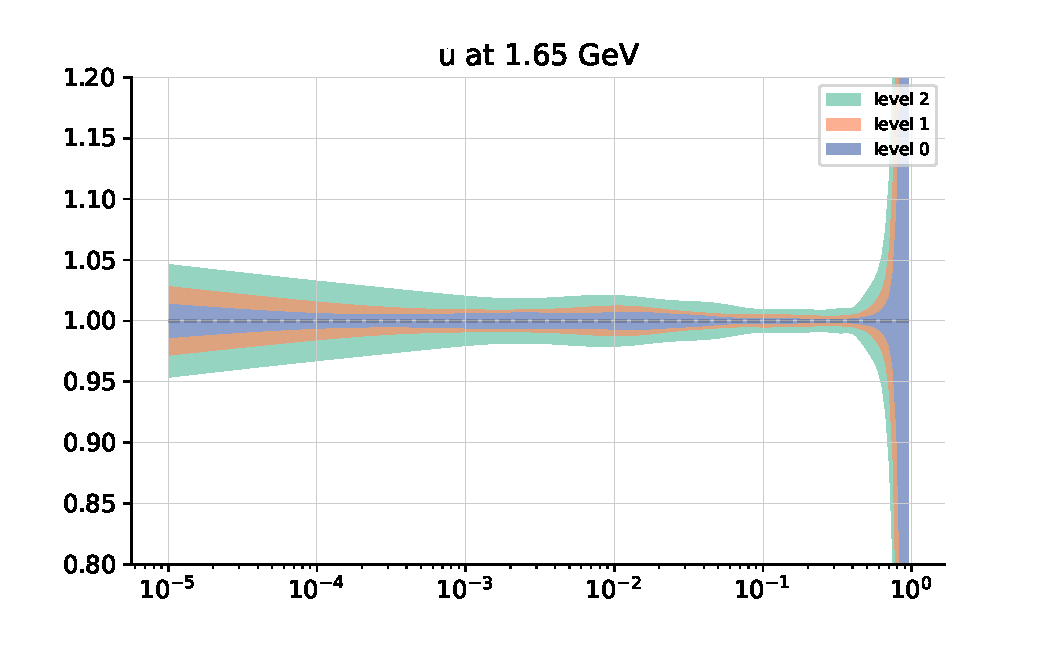
\includegraphics[scale=0.43]{CT_log_u.pdf}
    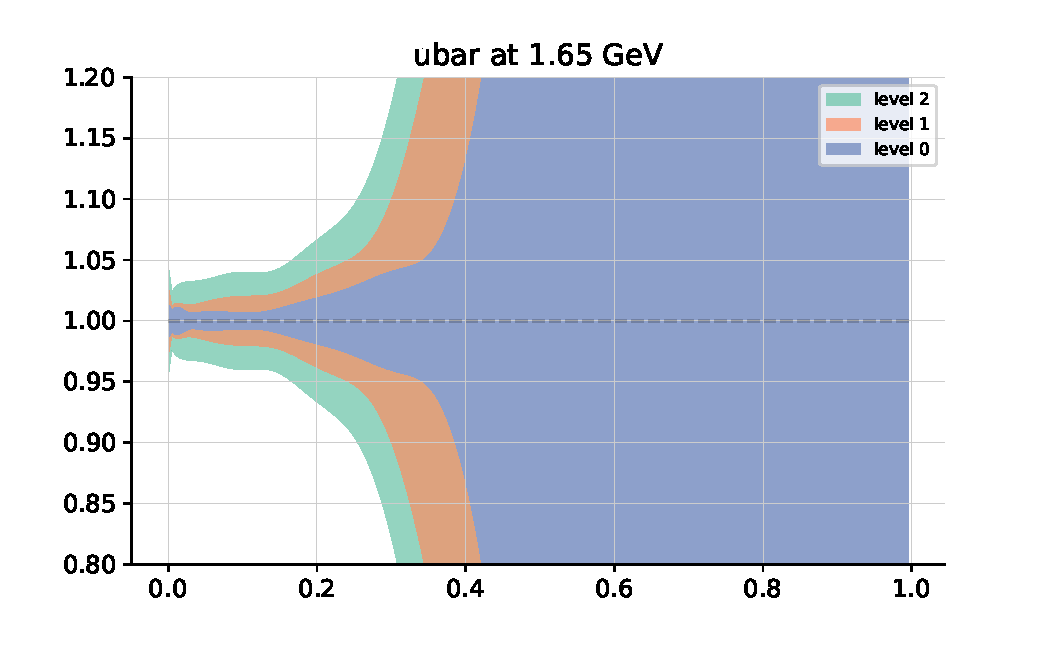
\includegraphics[scale=0.43]{CT_linear_ubar.pdf}
    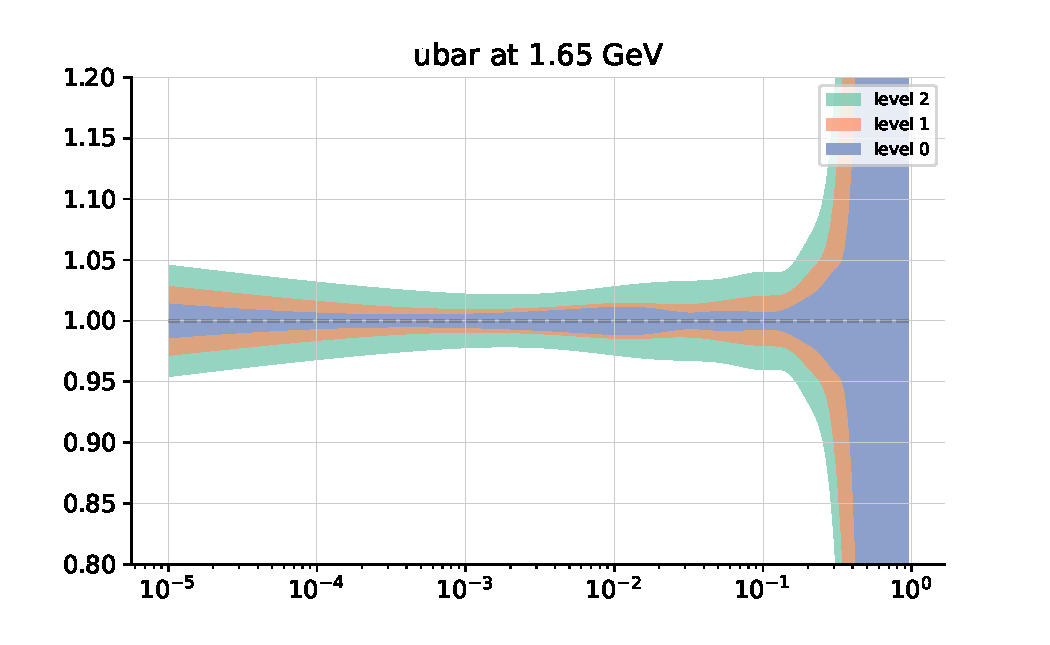
\includegraphics[scale=0.43]{CT_log_ubar.pdf}
    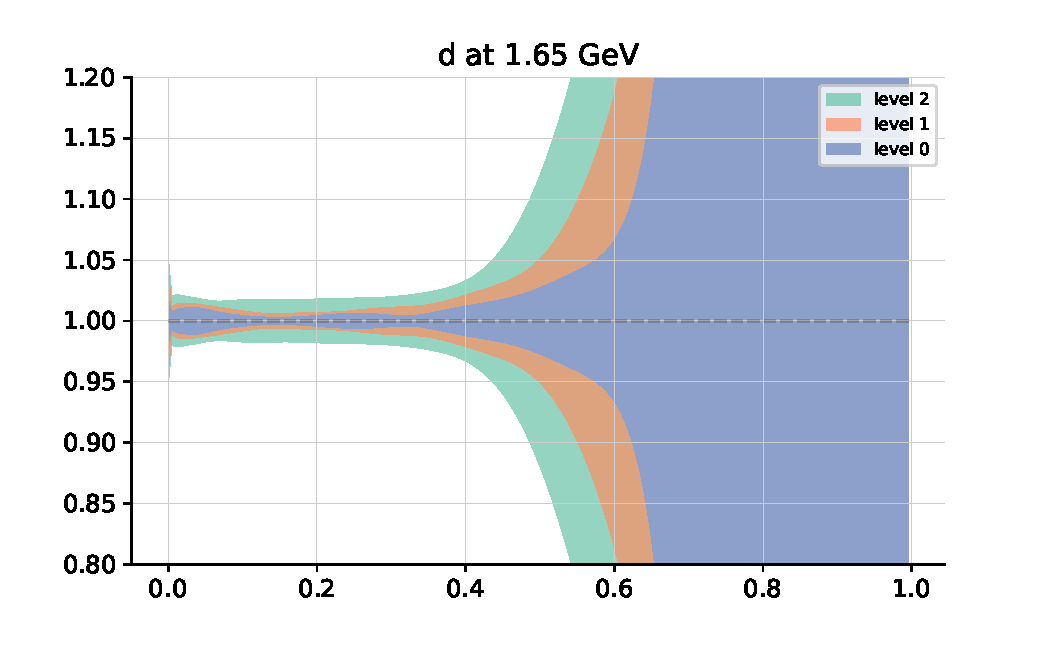
\includegraphics[scale=0.43]{CT_linear_d.pdf}
    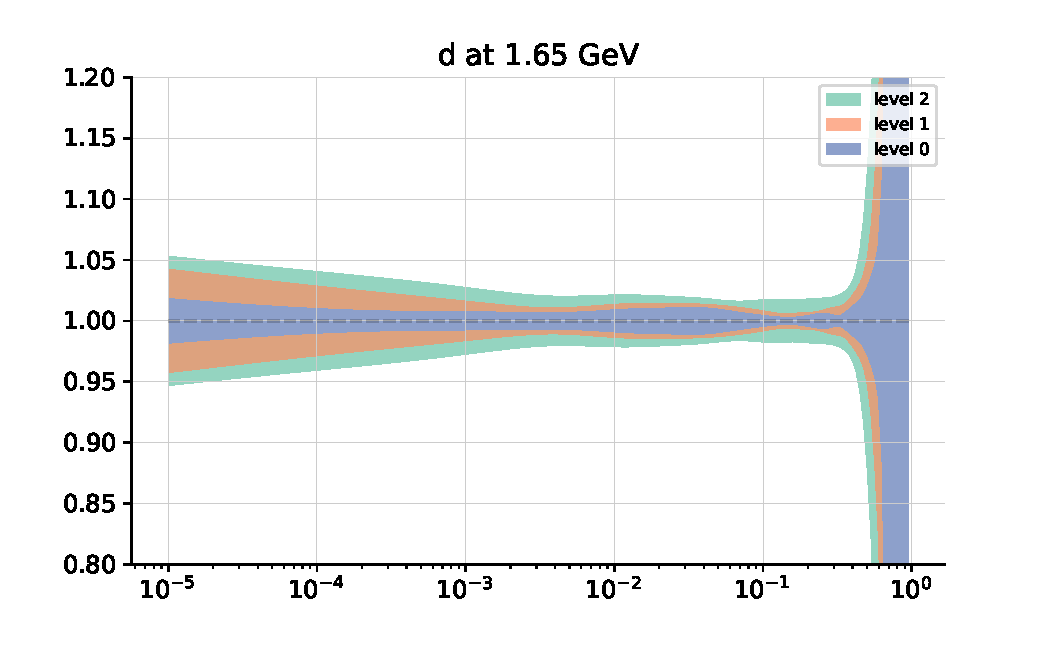
\includegraphics[scale=0.43]{CT_log_d.pdf}
    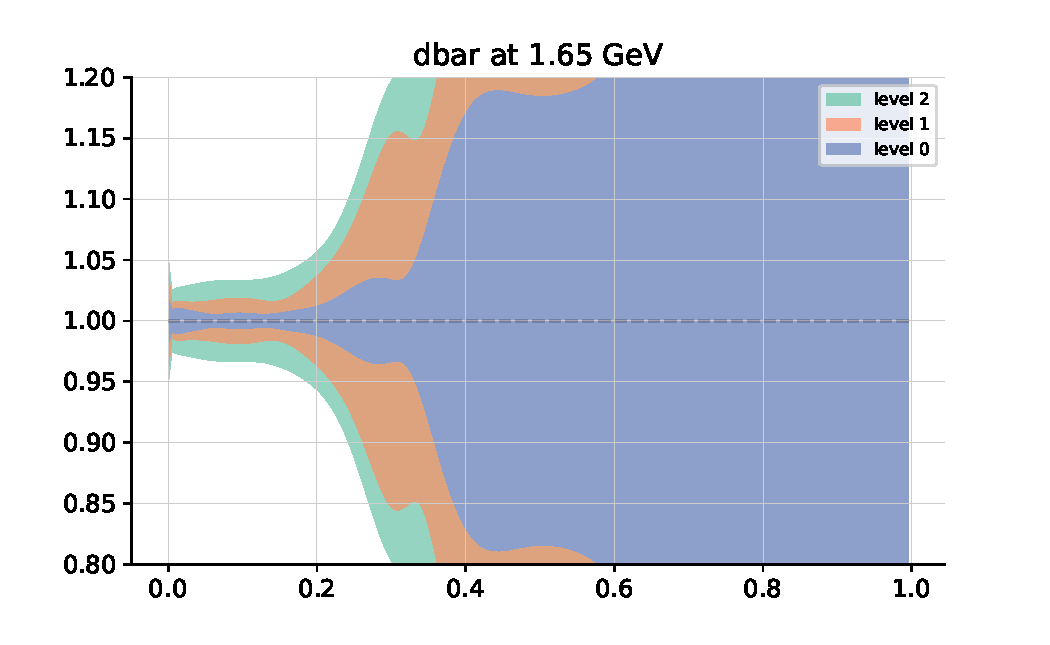
\includegraphics[scale=0.43]{CT_linear_dbar.pdf}
    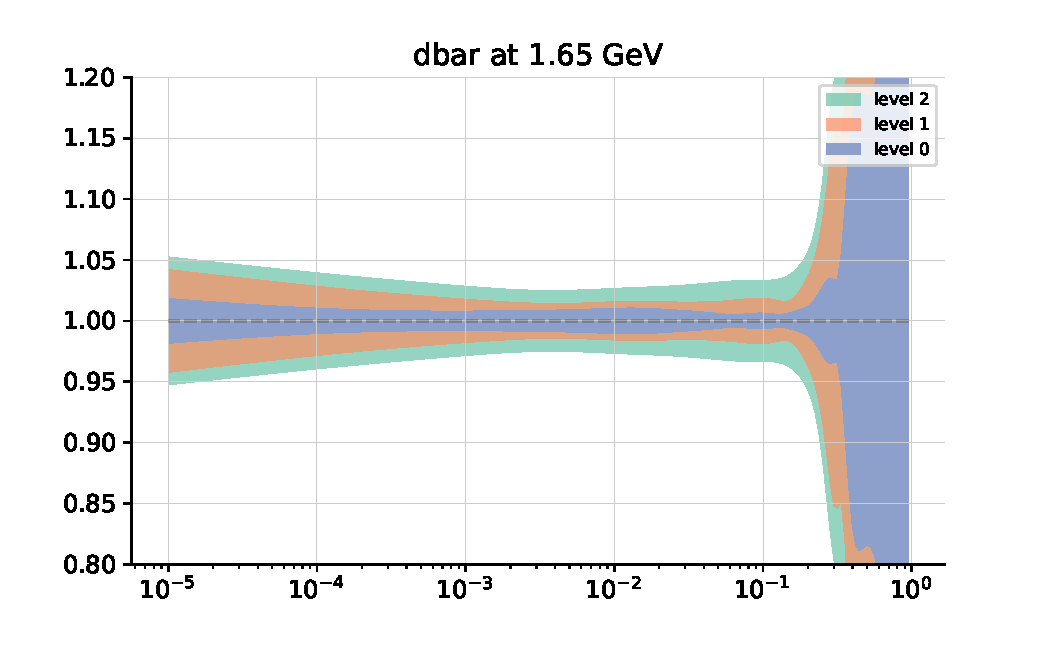
\includegraphics[scale=0.43]{CT_log_dbar.pdf}
    \caption{Results from L0, L1 and L2 closure tests for the $u$, $\bar{u}$, $d$ and $\bar{d}$ distributions in the new methodology,
    plotted in logarithmic (left) and linear scale (right). Each fit is normalized to its central value.}
    \label{fig:nnpdf40_ct_errors1}    
\end{figure}


\begin{figure}[ht]
    \centering
    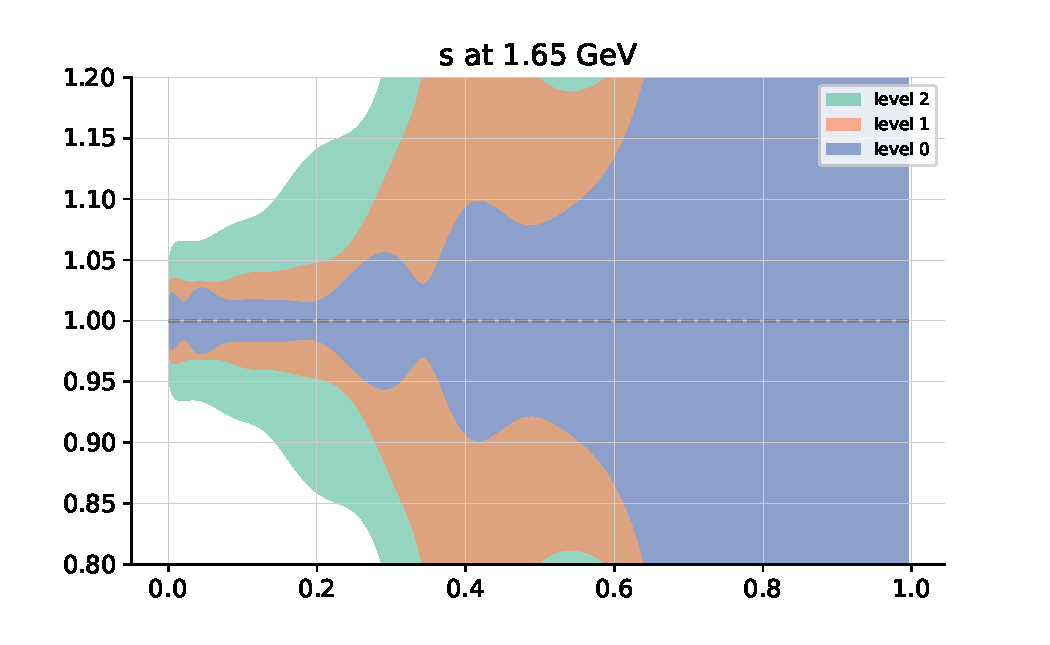
\includegraphics[scale=0.43]{CT_linear_s.pdf}
    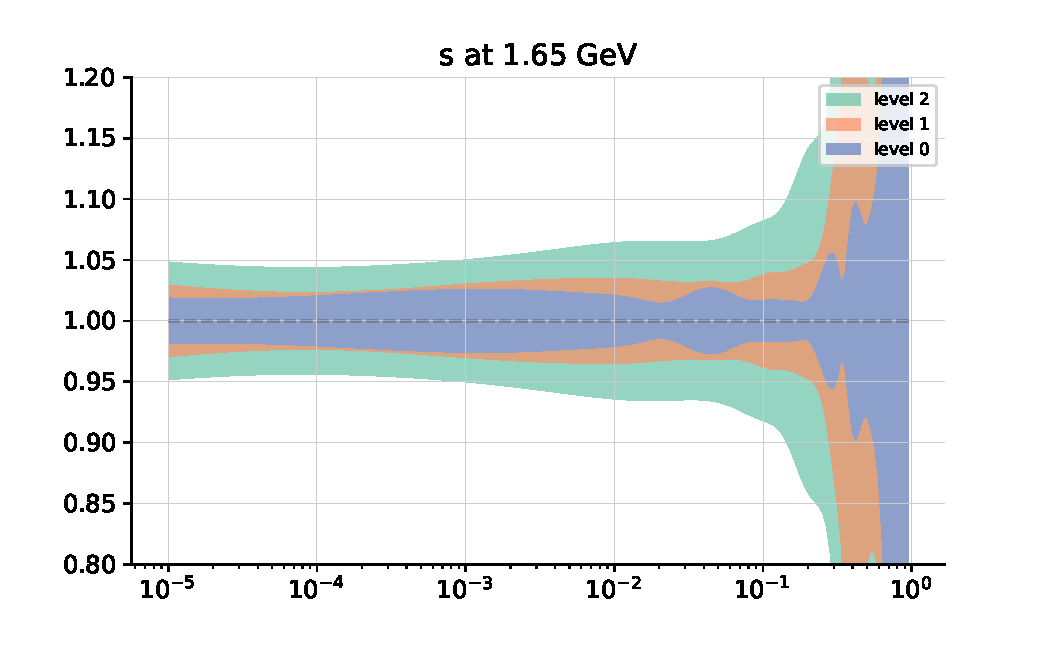
\includegraphics[scale=0.43]{CT_log_s.pdf}
    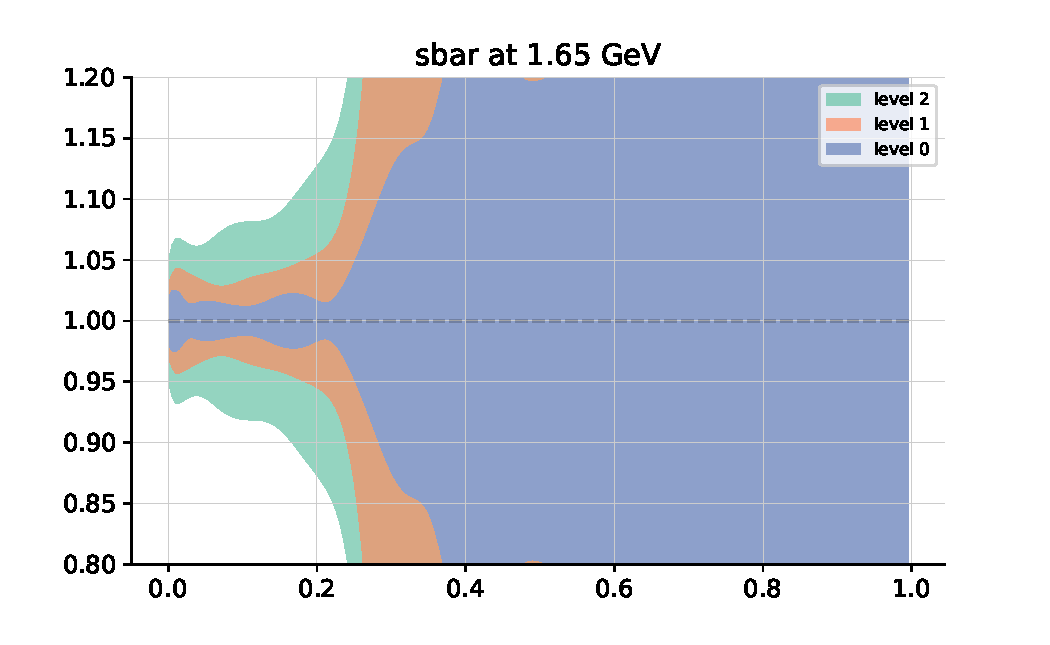
\includegraphics[scale=0.43]{CT_linear_sbar.pdf}
    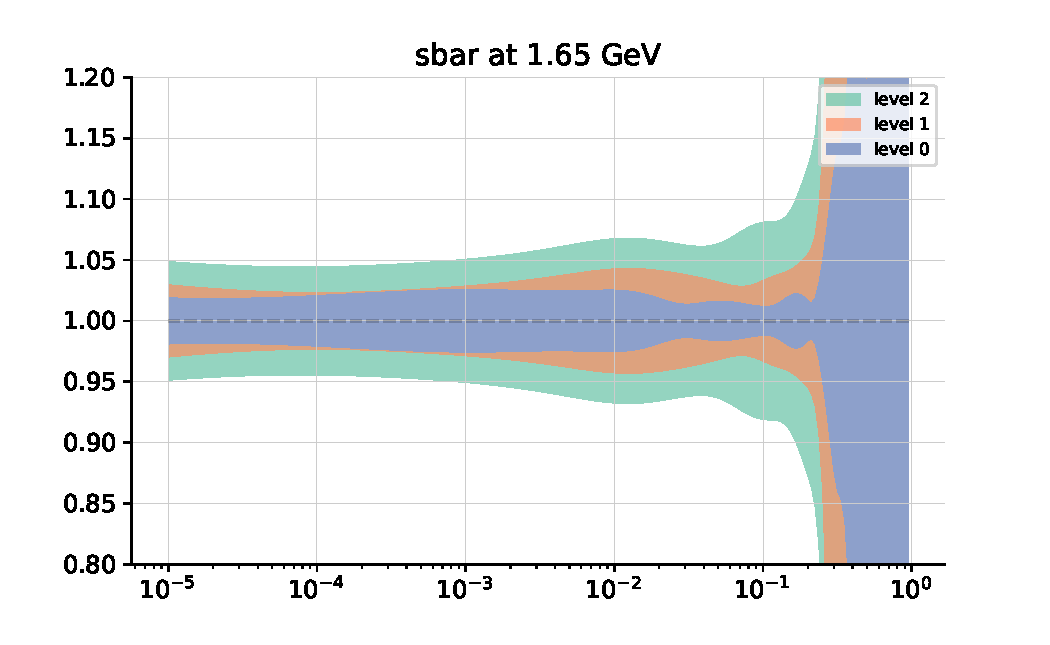
\includegraphics[scale=0.43]{CT_log_sbar.pdf}
    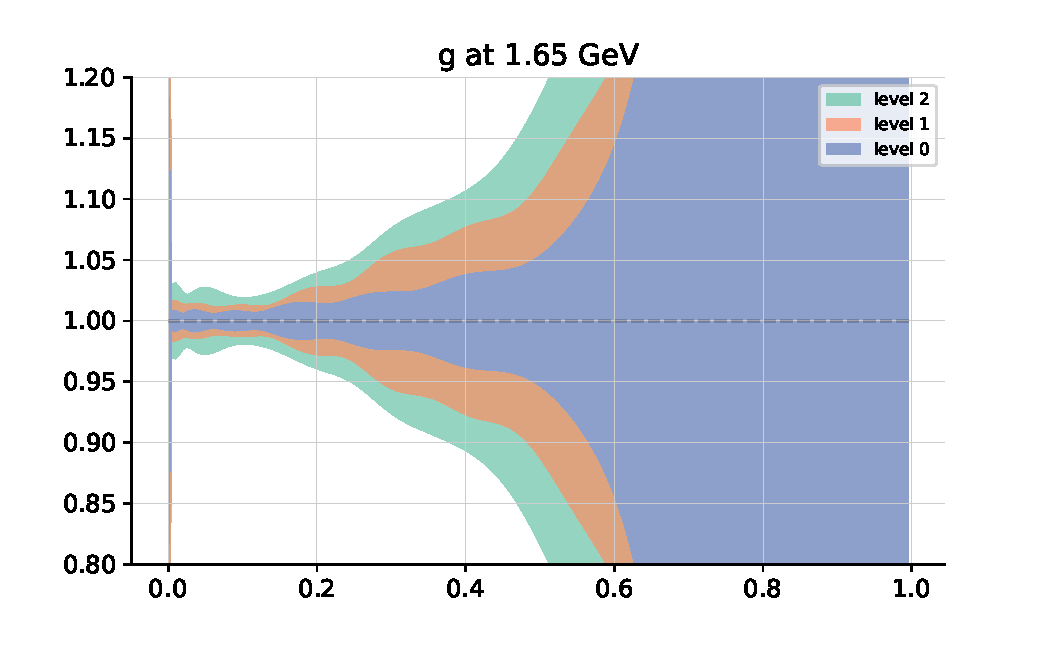
\includegraphics[scale=0.43]{CT_linear_g.pdf}
    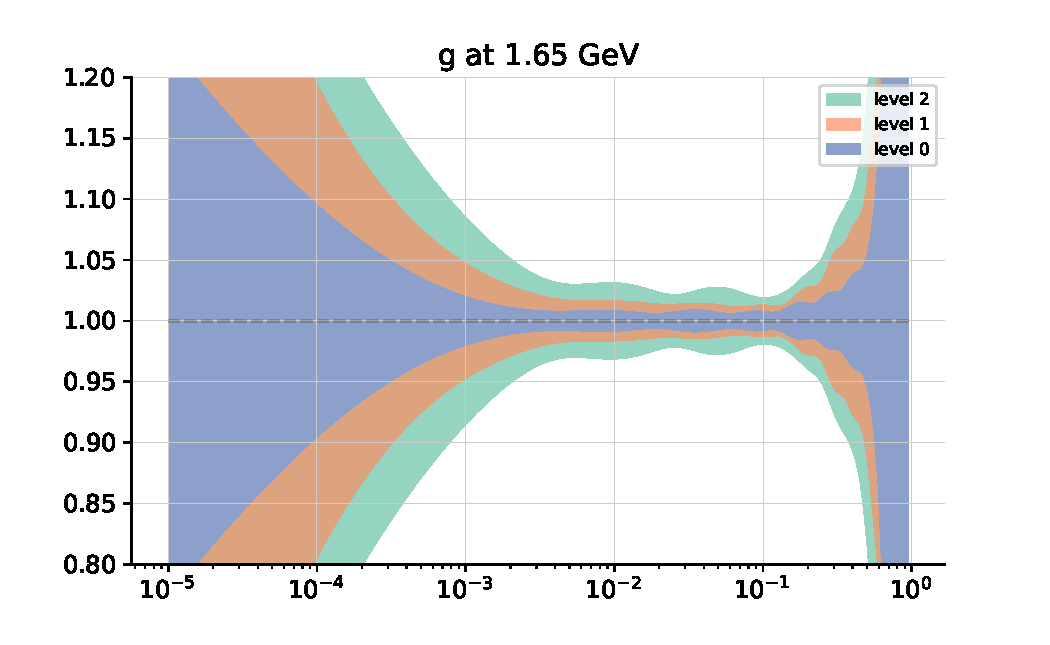
\includegraphics[scale=0.43]{CT_log_g.pdf}
    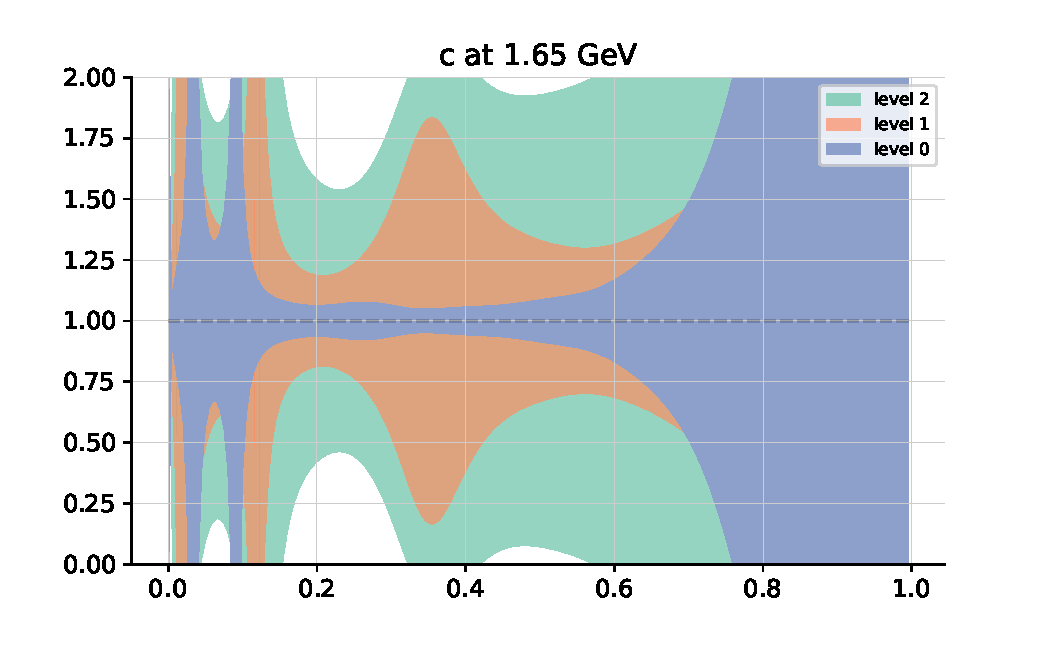
\includegraphics[scale=0.43]{CT_linear_c.pdf}
    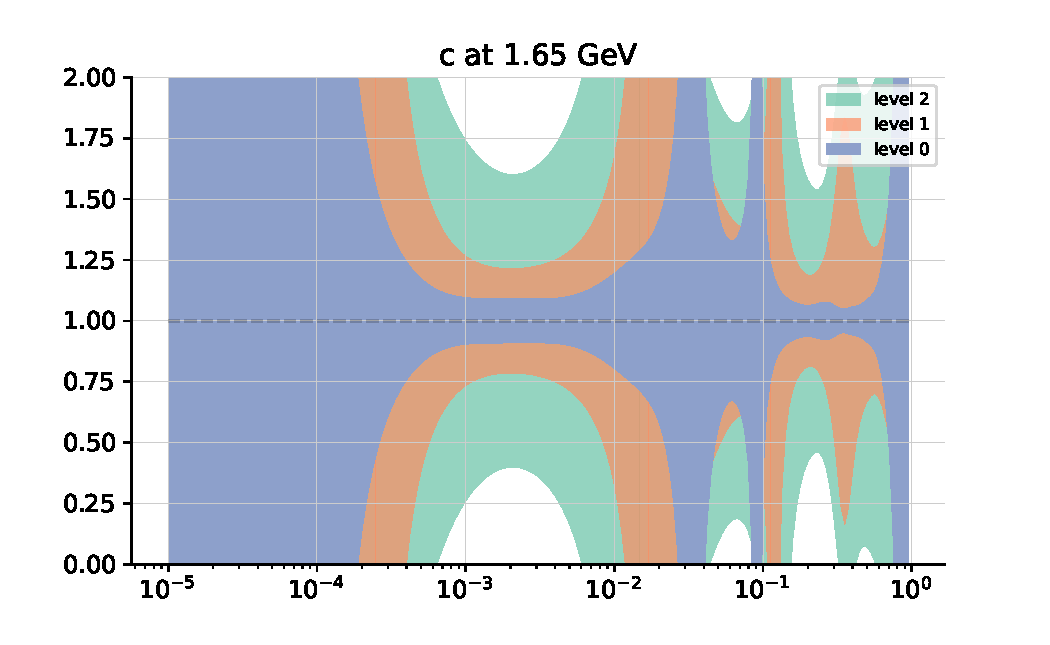
\includegraphics[scale=0.43]{CT_log_c.pdf}
    \caption{Same as Fig.~\ref{fig:nnpdf40_ct_errors1} but for the $s$, $\bar{s}$, $g$ and $c$ distributions .}
    \label{fig:nnpdf40_ct_errors2}    
\end{figure}

\begin{figure}[ht]
    \centering
    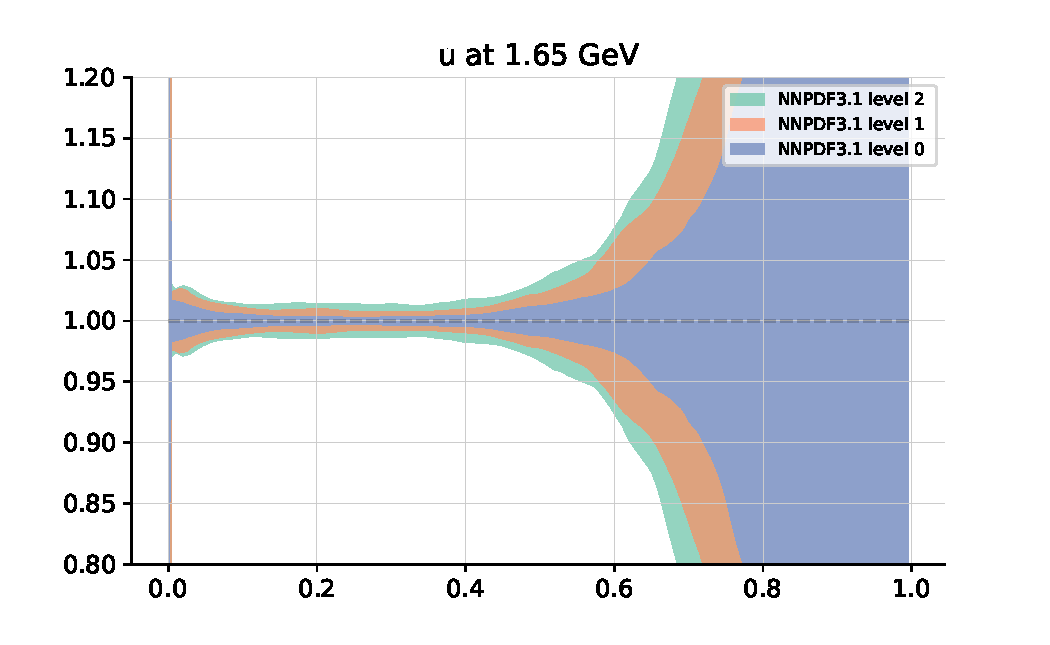
\includegraphics[scale=0.43]{CT_linear_u_nnpdf31.pdf}
    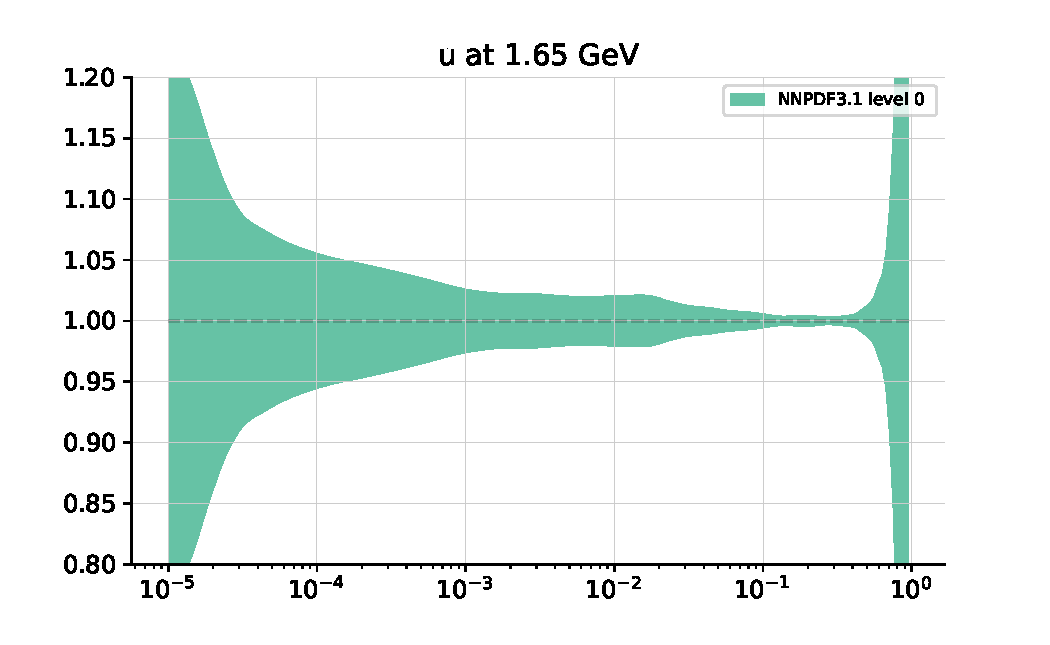
\includegraphics[scale=0.43]{CT_log_u_nnpdf31.pdf}
    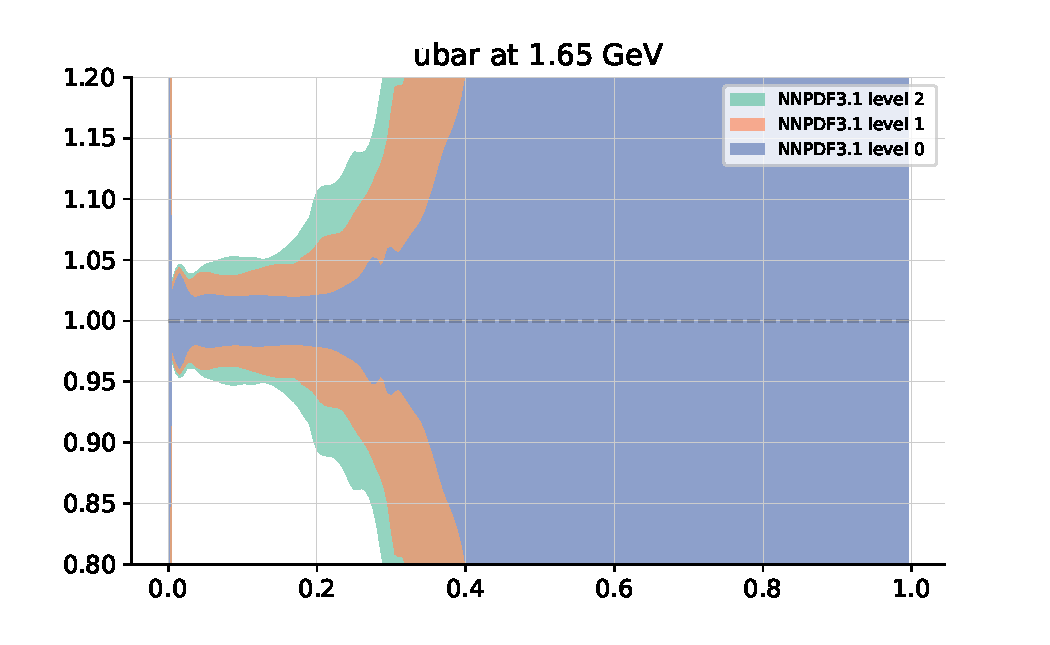
\includegraphics[scale=0.43]{CT_linear_ubar_nnpdf31.pdf}
    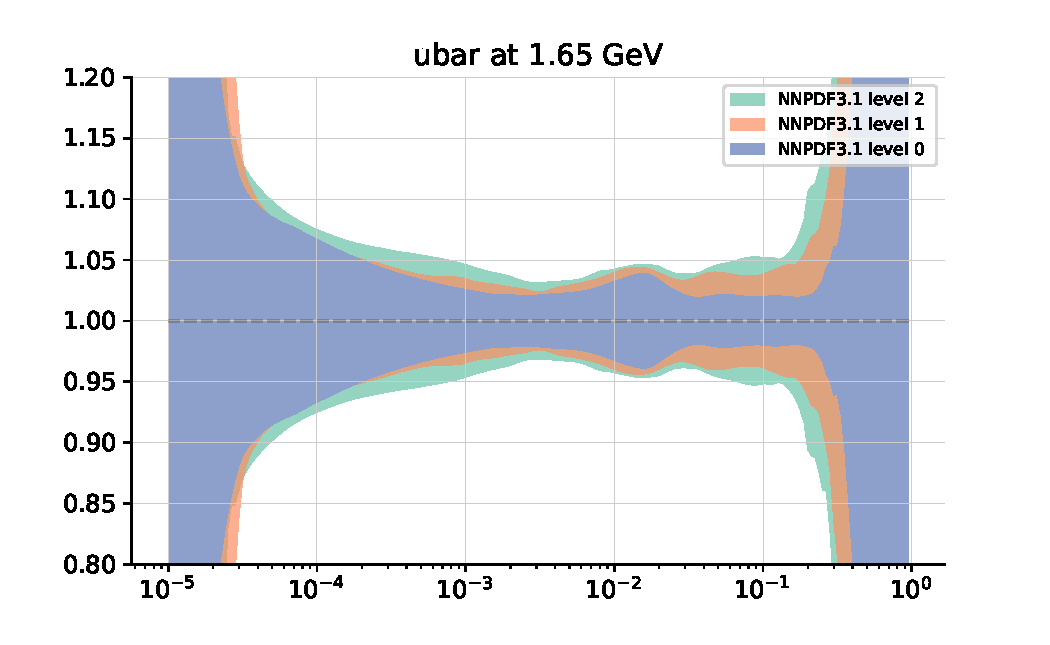
\includegraphics[scale=0.43]{CT_log_ubar_nnpdf31.pdf}
    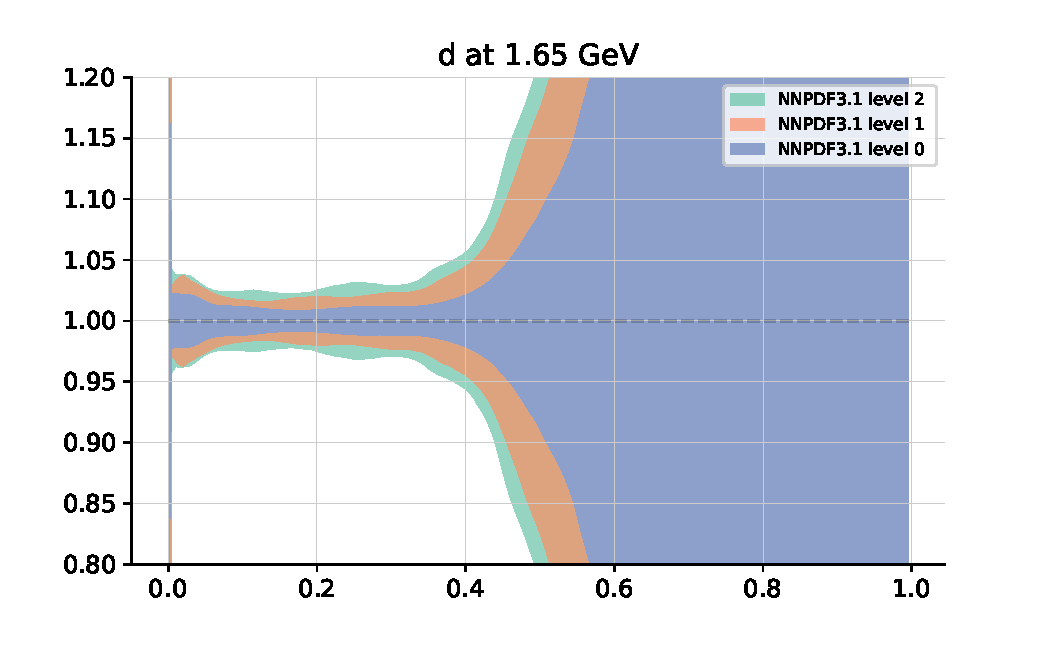
\includegraphics[scale=0.43]{CT_linear_d_nnpdf31.pdf}
    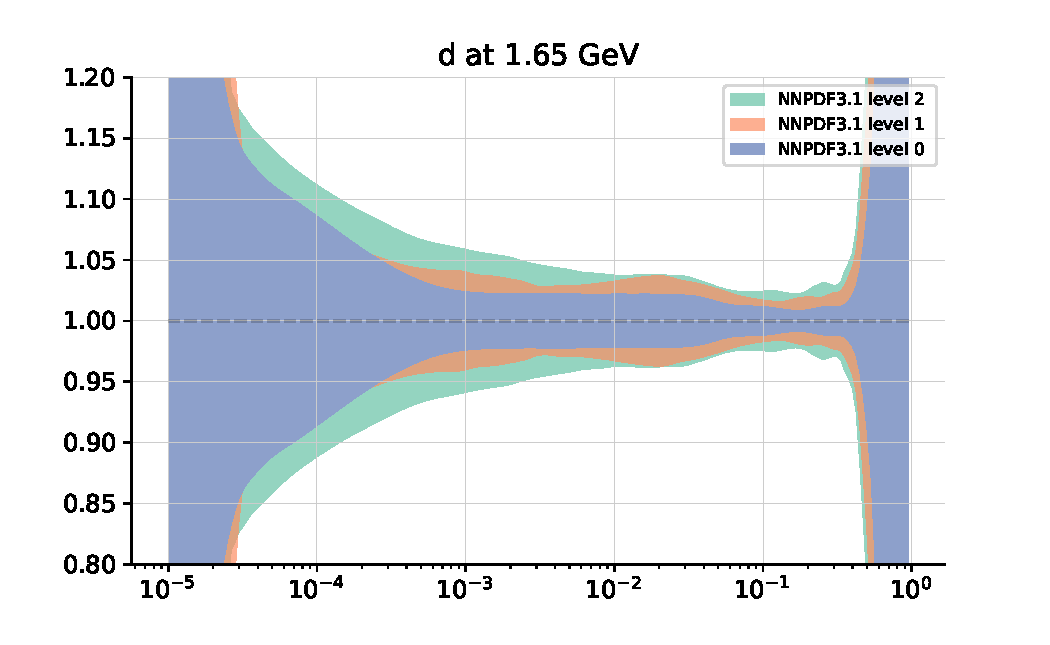
\includegraphics[scale=0.43]{CT_log_d_nnpdf31.pdf}
    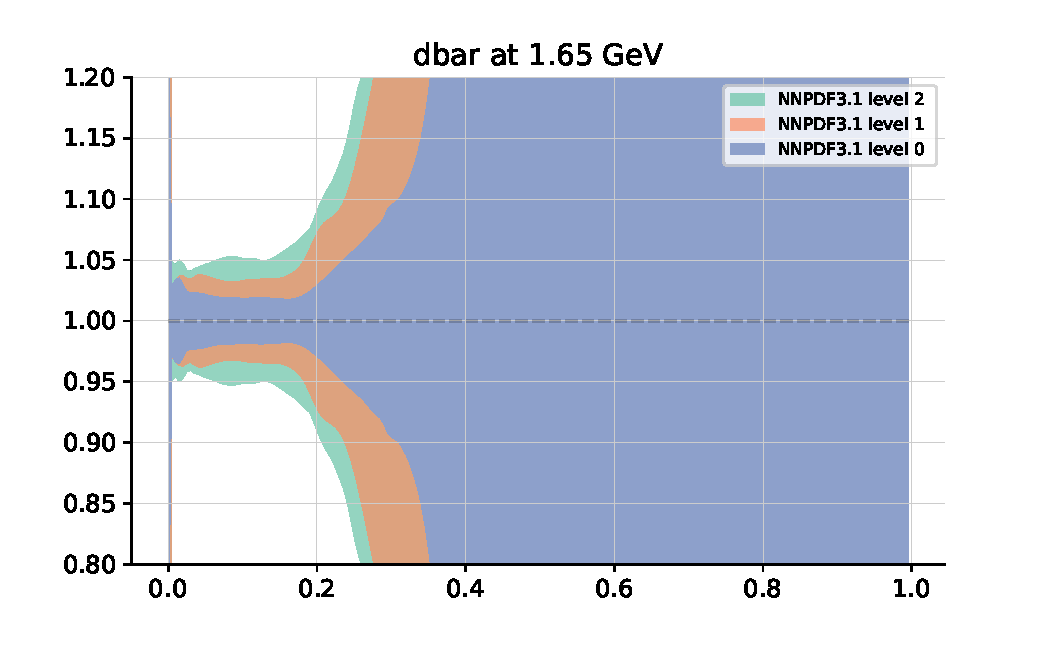
\includegraphics[scale=0.43]{CT_linear_dbar_nnpdf31.pdf}
    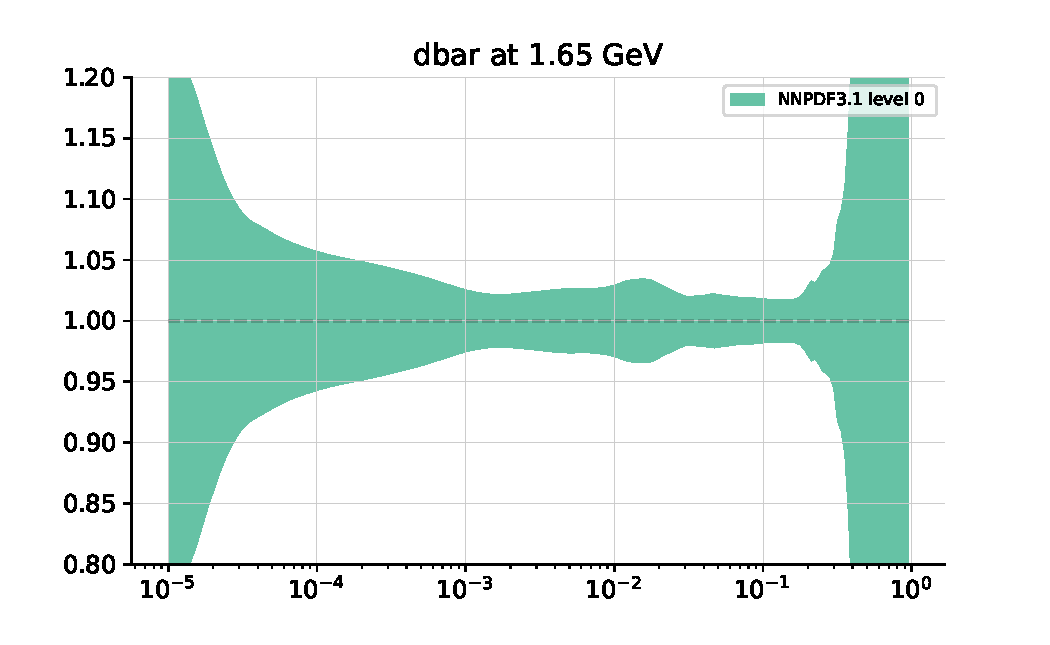
\includegraphics[scale=0.43]{CT_log_dbar_nnpdf31.pdf}
    \caption{Same as Fig.~\ref{fig:nnpdf40_ct_errors1} for the old methodology.}
    \label{fig:nnpdf31_ct_errors1}    
\end{figure}

\begin{figure}[ht]
    \centering
    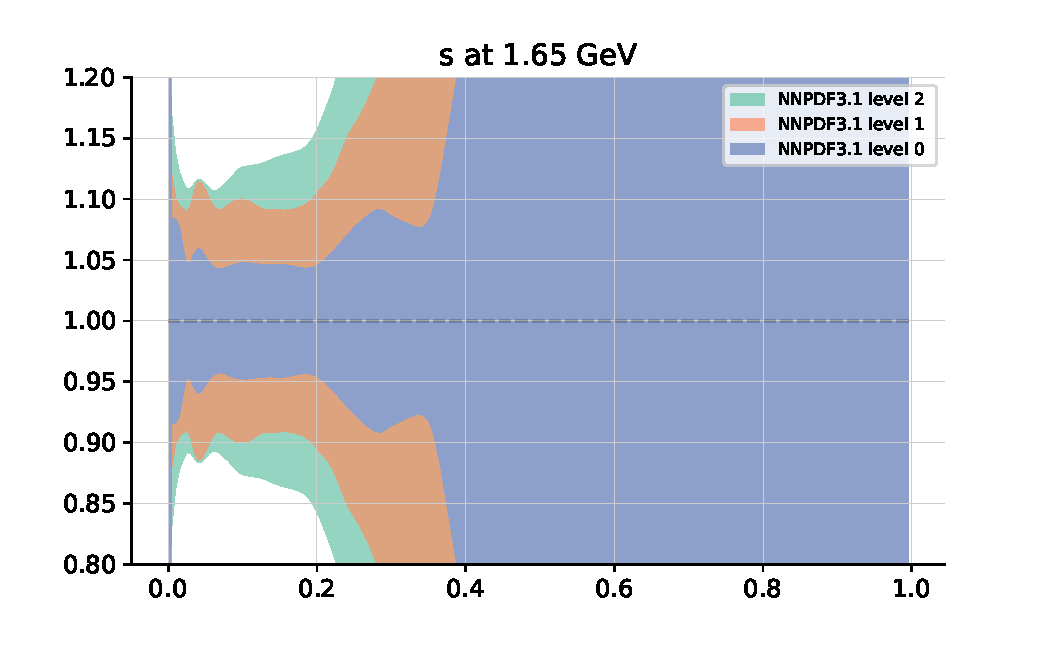
\includegraphics[scale=0.43]{CT_linear_s_nnpdf31.pdf}
    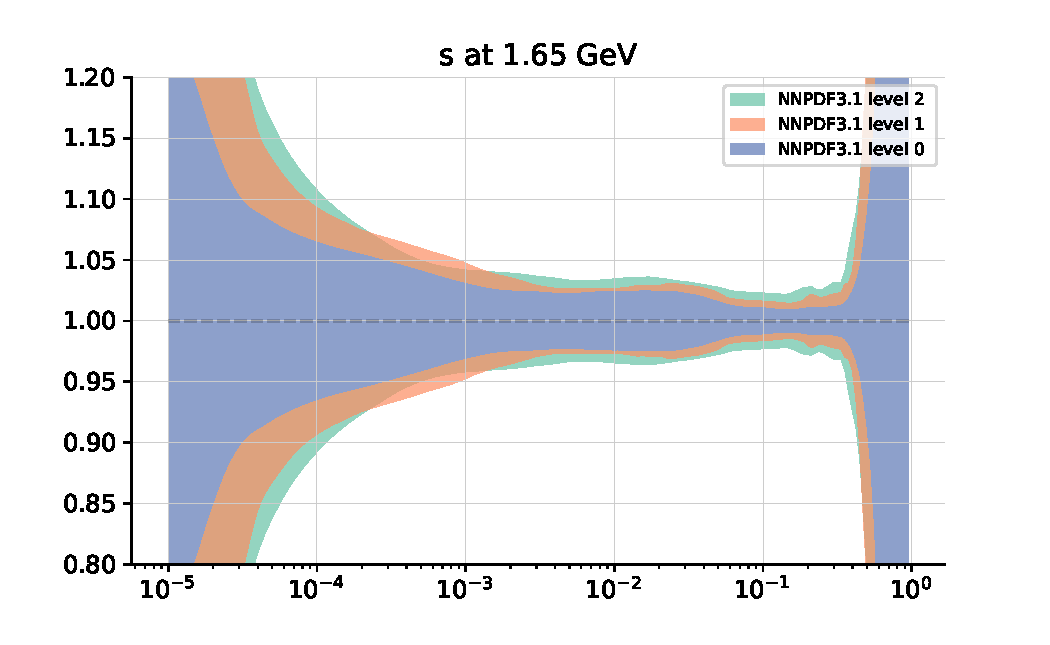
\includegraphics[scale=0.43]{CT_log_s_nnpdf31.pdf}
    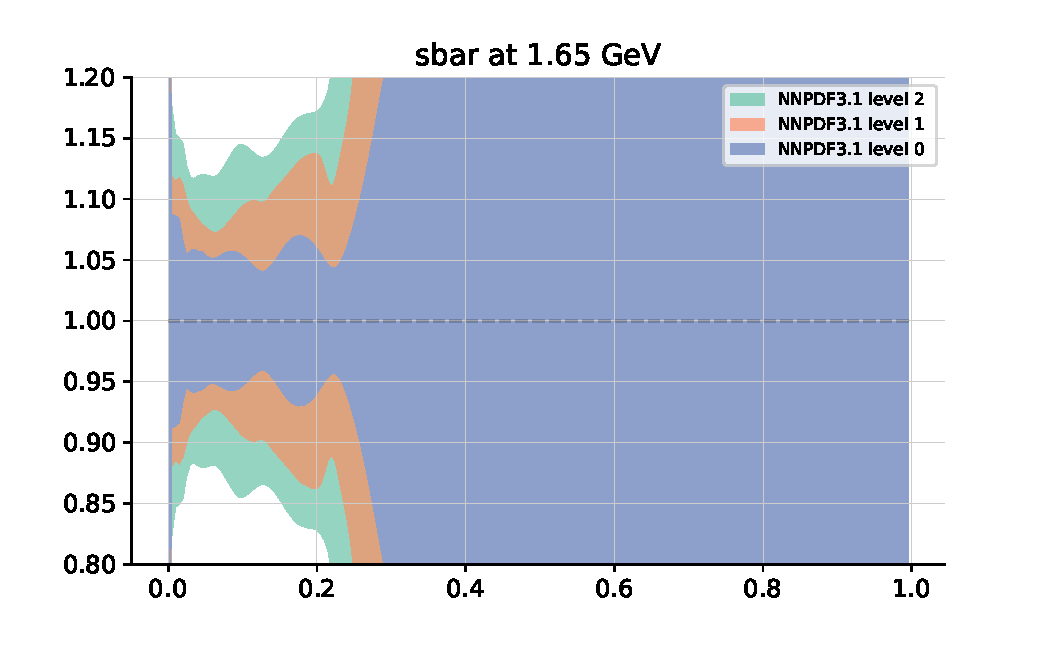
\includegraphics[scale=0.43]{CT_linear_sbar_nnpdf31.pdf}
    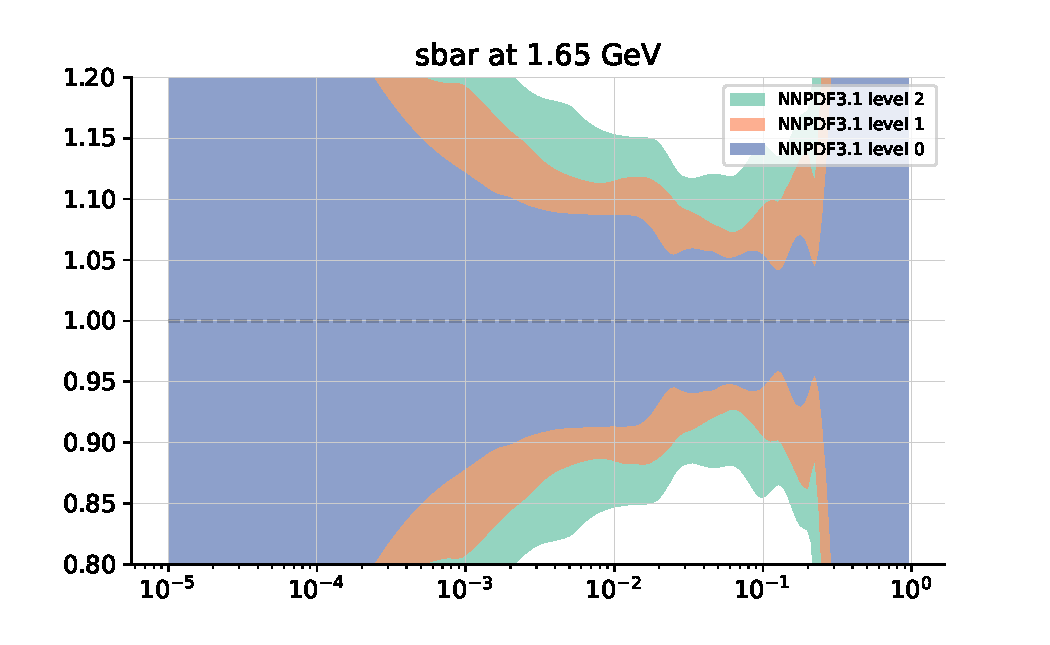
\includegraphics[scale=0.43]{CT_log_sbar_nnpdf31.pdf}
    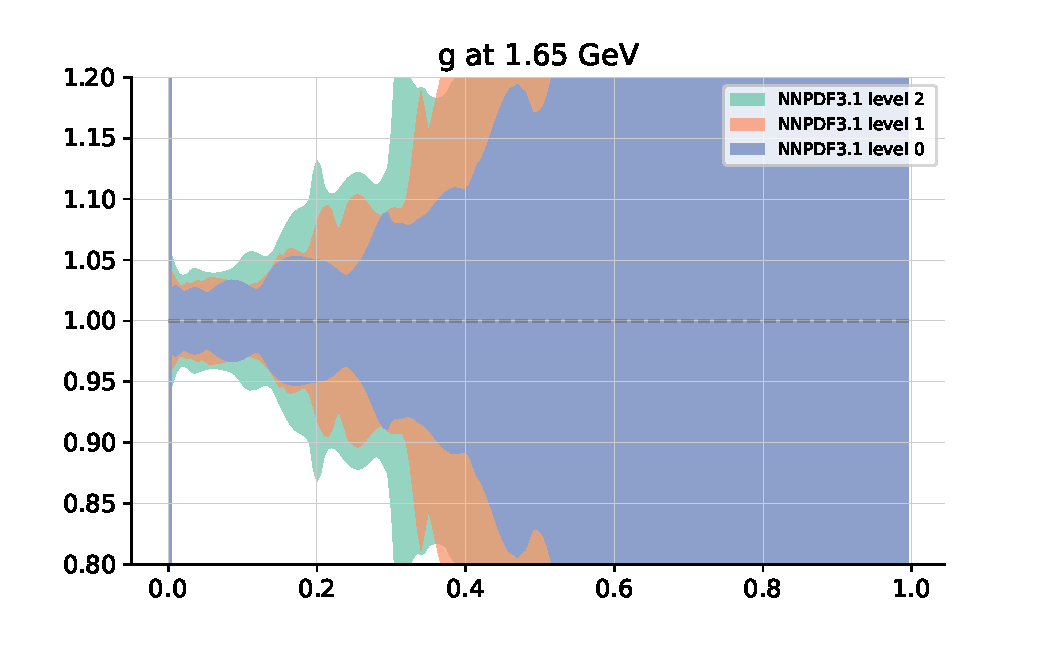
\includegraphics[scale=0.43]{CT_linear_g_nnpdf31.pdf}
    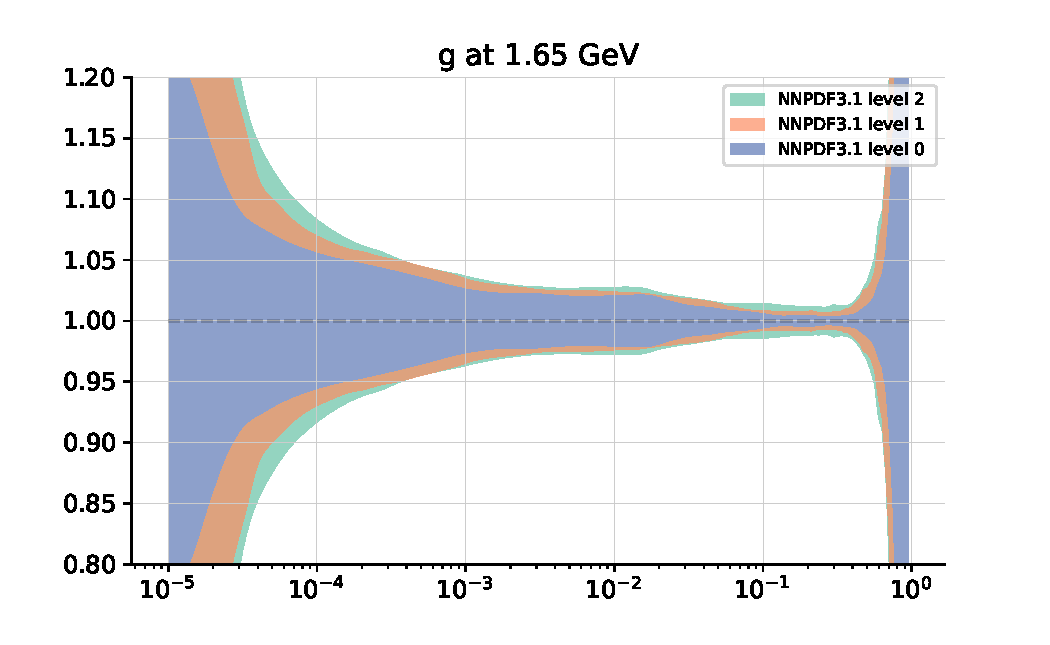
\includegraphics[scale=0.43]{CT_log_g_nnpdf31.pdf}
    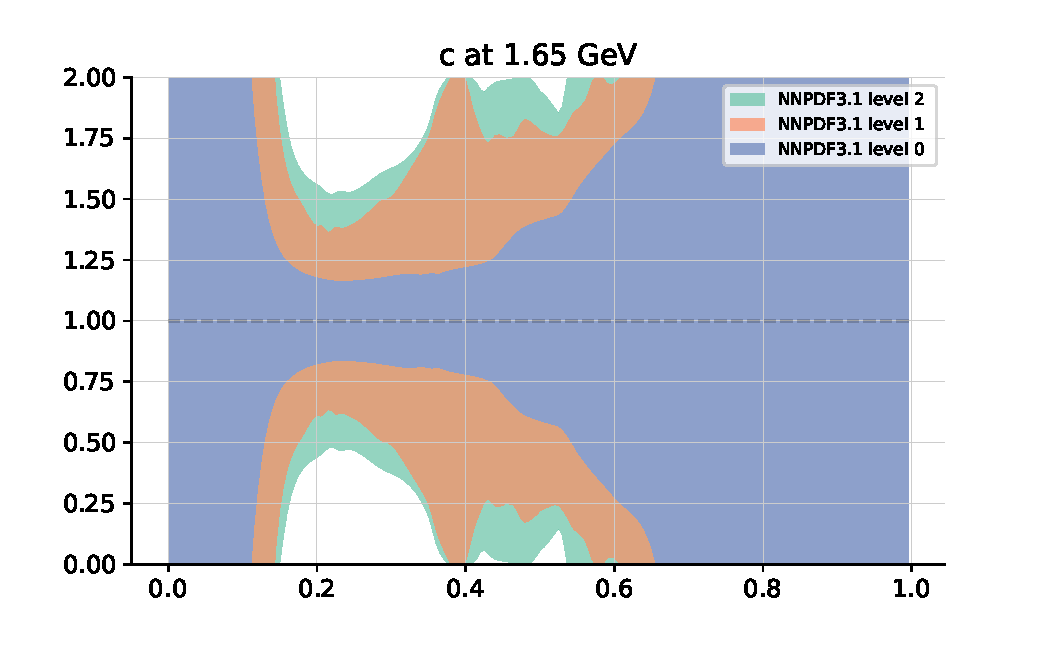
\includegraphics[scale=0.43]{CT_linear_c_nnpdf31.pdf}
    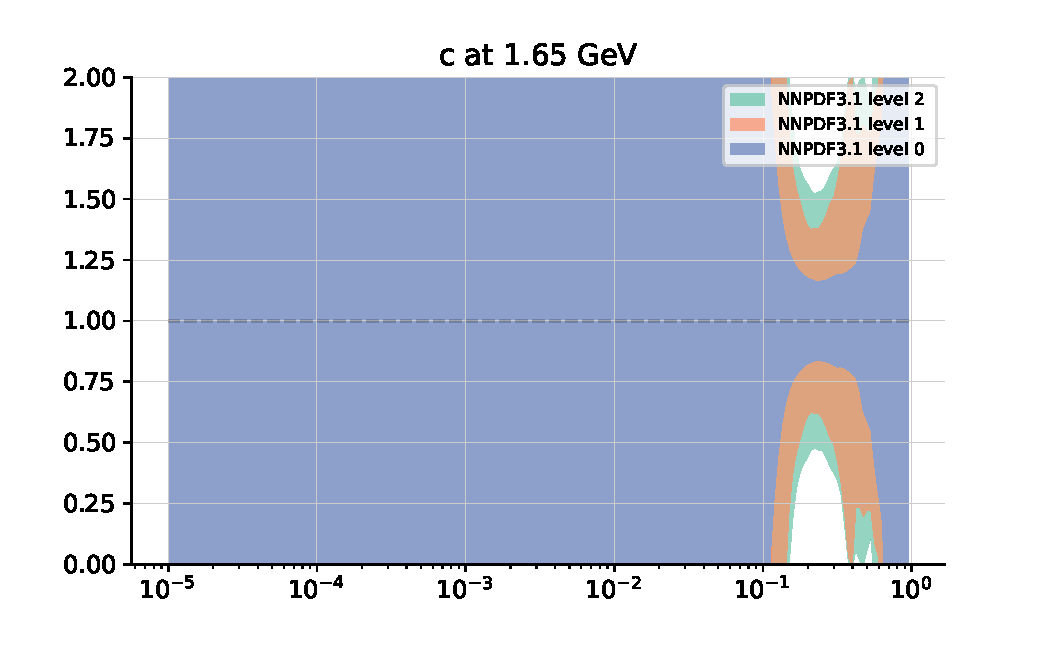
\includegraphics[scale=0.43]{CT_log_c_nnpdf31.pdf}
    \caption{Same as Fig.~\ref{fig:nnpdf40_ct_errors2} for the old methodology.}
    \label{fig:nnpdf31_ct_errors2}    
\end{figure}
\fi
